\section{Industrial Robots}
\subsection{History of Industrial Robots}
The idea of automatic machines has been in existence since many centuries with documented illustrations of robots, automata in various interesting applications. Archytas (4th century B.C), the founder of mathematical mechanics, invented an autonomous wooden flying pigeon powered by steam. Fig.~\ref{fig:automatons0} (a) shows this mechanical bird which can fly uninterrupted for hundreds of meters and is considered to be the first ever robot documented. Another interesting application shown in Fig.~\ref{fig:automatons0} (b) is an analog computer (developed during 1st century B.C) that can predict astronomical positions for the purpose of maintaining a calendar and astrological reasons. It has 37 gears enabling the device to track the moon and sun positions keeping track of time. Hydro powered clocks was common in China since the 40th century B.C to study astronomical positions. Fig.~\ref{fig:automatons0} (c) shows Su Song's artistic clock tower developed in 10th century A.D with mechanically controlled mannequins chiming and ringing bells. Al Jazari in the muslim world is known for developing hydro powered automatic machines such as the drink-serving waitress, hand washing automaton, peacock fountain. Though it might look trivial, the works were known for its creative mechanisms, components and design features. Cam \& crank shafts, escapement mechanism in rotating wheels, segmental gears are some of his contributions which are still used in modern mechanical devices today \cite{hill2012book}.  

\begin{figure*}[!tbph]
\begin{subfigure}
[Archytas' bird]{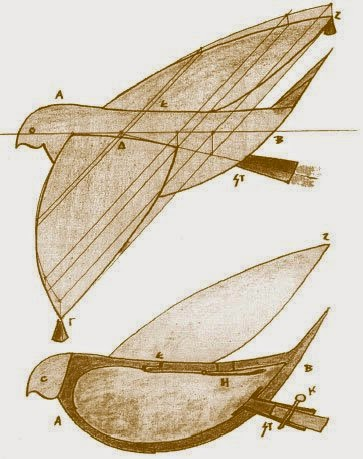
\includegraphics[width=4.1cm,height=5.5cm]{chapters/intro/images/pigionsteam.jpg}}\quad
\end{subfigure}
\begin{subfigure}
[Antikythera mechanism]{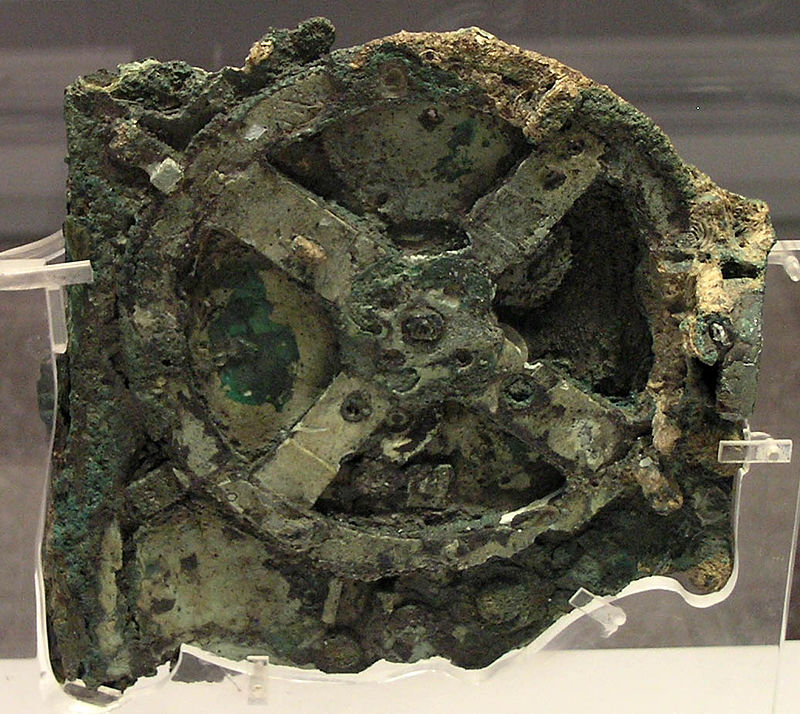
\includegraphics[width=4.3cm,height=5.5cm]{chapters/intro/images/machineanti.jpg}}\quad
\end{subfigure}
\begin{subfigure}
[Su Song's Clock Tower]{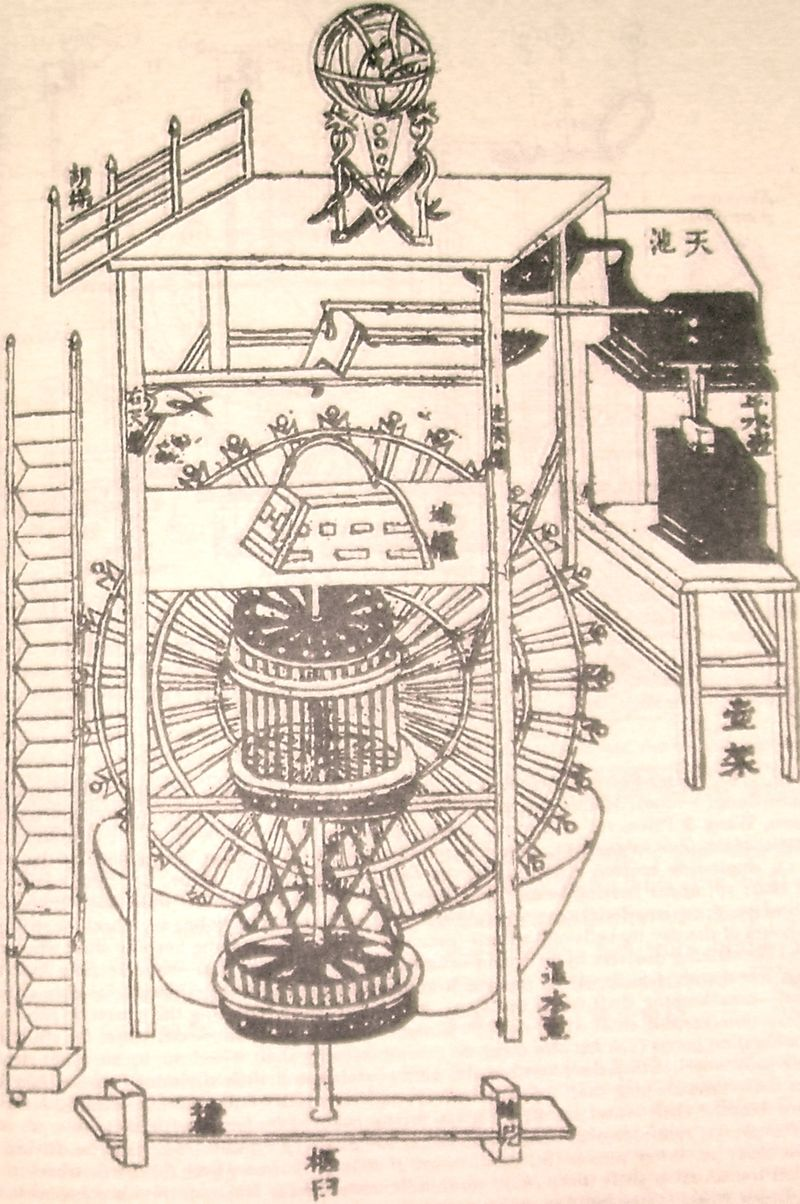
\includegraphics[width=4.1cm,height=5.5cm]{chapters/intro/images/clocktower.JPG}}\quad
\end{subfigure}
\caption{Automatons in the ancient world}
\label{fig:automatons0}
\end{figure*}

Fig.~\ref{fig:automatons1} (a) shows the first ever humanoid robot in the records, designed by Leonardo da Vinci. This mechanical knight has joints similar to human beings with an ability to perform motions such as waving the arms, moving the head and jaws, sitting and standing up. Around 18th century many automatons were developed capable of entertaining, speaking and playing musical instruments. One such musical automaton in the form of an elephant shown in the Fig.~\ref{fig:automatons1} (b) is designed by Hubert Martinet, a french clockmaker in 1774. Another interesting automaton in the Fig.~\ref{fig:automatons1} (c) is the \textit{Digesting Duck} made by Jacques de Vaucanson. This golden mechanical duck imitates the ability to eat and defecate grains.

\begin{figure*}[!tbph]
\begin{subfigure}
[Da Vinci's robot]{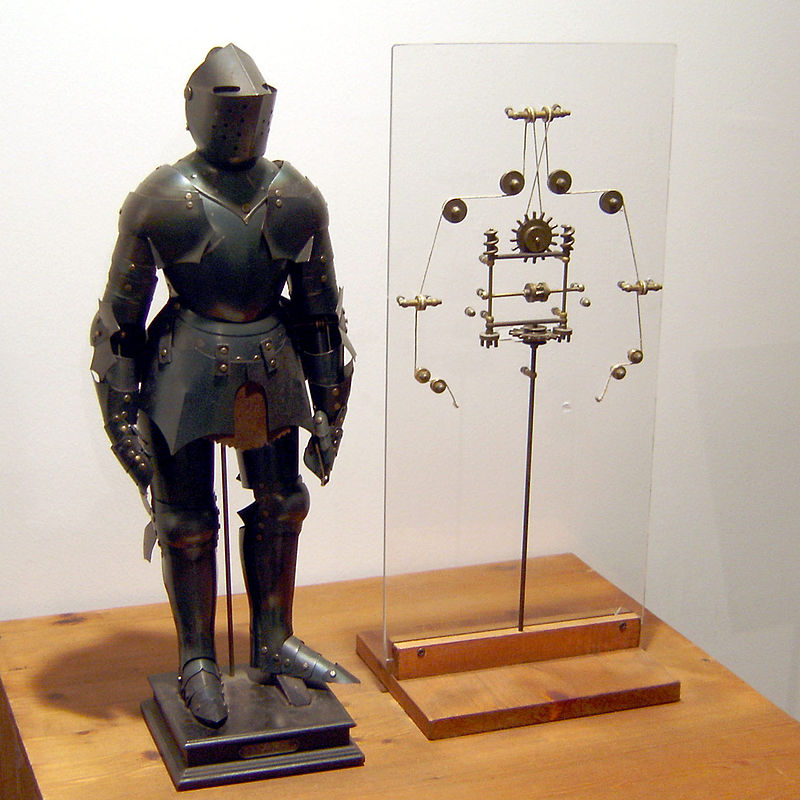
\includegraphics[width=4cm,height=4.5cm]{chapters/intro/images/leorobot.jpg}}\quad
\end{subfigure}
\begin{subfigure}
[Elephant Automaton]{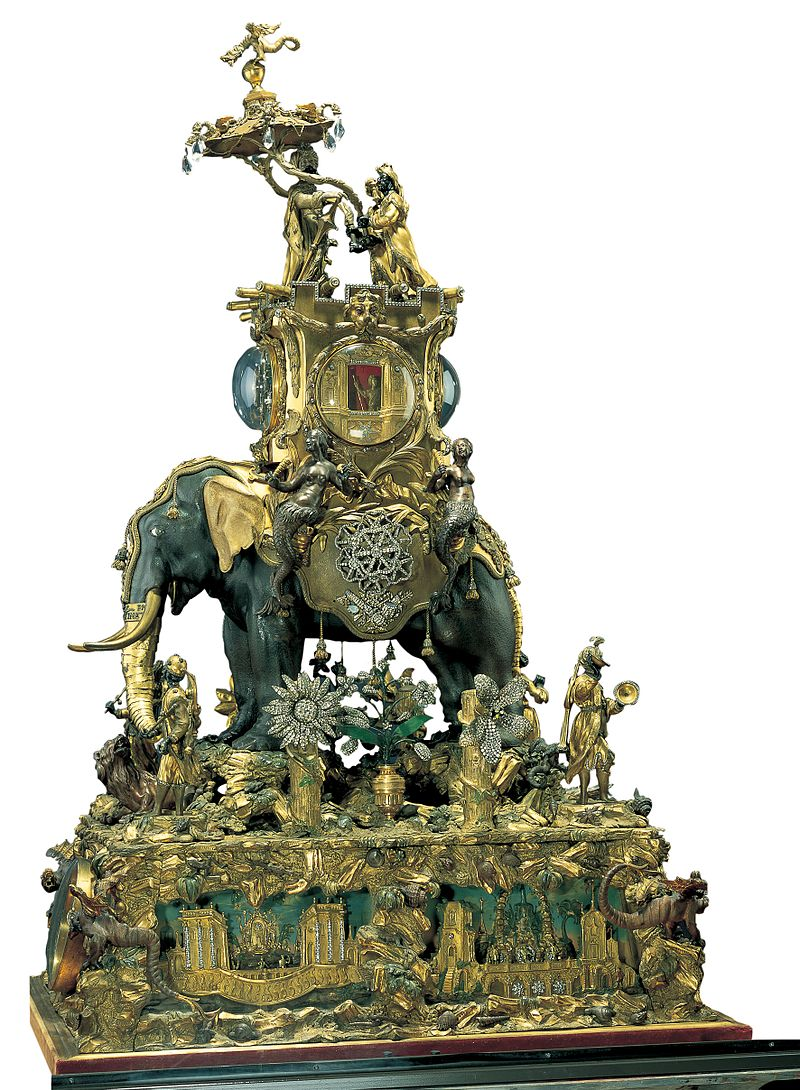
\includegraphics[width=4cm,height=4.5cm]{chapters/intro/images/elephantAutomaton.jpg}}\quad
\end{subfigure}
\begin{subfigure}
[Digesting Duck]{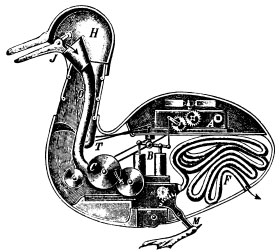
\includegraphics[width=4cm,height=4.5cm]{chapters/intro/images/duck.jpg}}\quad
\end{subfigure}
\caption{Automatons in the 18th Century}
\label{fig:automatons1}
\end{figure*}

% May be talk about Remote-controlled systems

Though most of the automatons were created for fun or artistic satisfaction in the beginning, the characterization of robots to be human look-alike machines that can serve human beings came up in the 20th century. The term \textit{robot} itself was born in 1921 from R.U.R (Rossum's Universal Robots), a czech play written by Karel Čapek. The play depicts robots as good and benevolent workers serving the human beings later gaining super human strength to revolt humans leading to end of life. This negative idea changed after a russian writer, Isaac Asimov made a contrasting characterization of robots as just mechanical creatures with no emotions. Asimov's laws of robotics in 1942 gave way to a new perspective of robots to be seen as an product that could be developed by engineers to improve productivity in manufacturing industries. During the same time period, a programmable mechanism to do spray painting was designed by Pollard and Roselund for DeVilbiss, the first industrial robot supplier. The mechanism is based on pantograph pivoted on two rotary actuators on a fixed base. 


\begin{figure*}[!tbph]
\centering
\begin{subfigure}
[Pollard's Paint Sprayer]{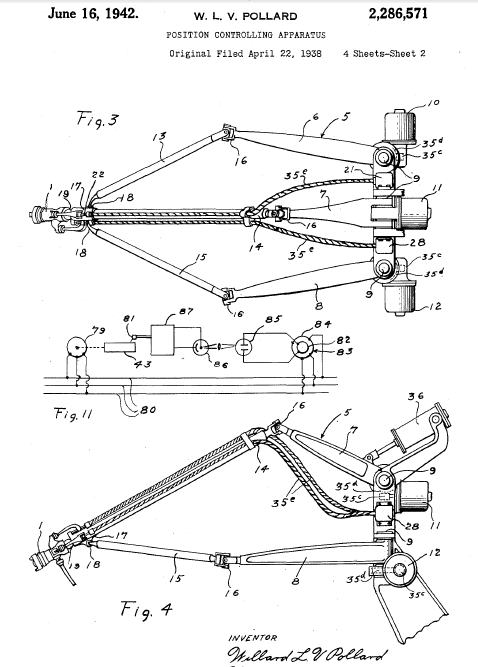
\includegraphics[width=6.5cm,height=6cm]{chapters/intro/images/pollard.png}}
\end{subfigure}
\begin{subfigure}
[Unimate Robot's Television Appearance]{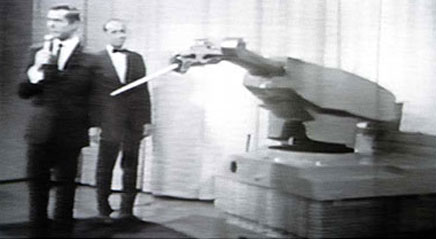
\includegraphics[width=6.5cm,height=6cm]{chapters/intro/images/unimate.jpg}}
\end{subfigure}
\caption{Robotic Mechanisms in the Beginning}
\label{fig:robotmechanisms}
\end{figure*}


In 1954, George Devol developed the the first truly programmable robot UNIMATE which originally consisted of an arm and a drum memory box with pre-programmed tasks. A collaboration with Joseph Engelberger, the father of robotics gave birth to \textit{Unimation}, the first company to make robots which were used to transport and weld die castings on auto bodies preventing humans from dangerous working conditions. Though the numerically controlled turning \& milling machines and the hydraulic assembly machines were programmable, the industrial robots differed in the sophistication of reprogrammability and the versatility to be used for different tasks. This is purely because of the invention of digital computers and integrated circuit technology which allowed to develop the brains of industrial robots.

\begin{figure}[h]
\centering
{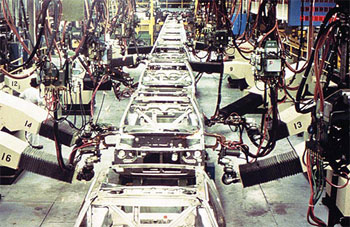
\includegraphics[scale=1]{chapters/intro/images/gm.jpg}}
\caption{Manufacturing unit in General Motors with 'Unimate' robots in 1969}
\label{fig:unimate}
\end{figure}

Ford director Del Harder's interest to install 2000 unimation robots triggered American manufacturing industries to pay attention to the robotics industry a bit more seriously. Installations in General Motors in Ohio, US in the beginning of 1960s marks the real beginning of industrial robotics. After an intense research and development during the next 15 years and the introduction of micro-processors provided the basis for low cost control systems. A norwegian company \textit{Trallfa} designed and developed a cost-effective alternative to Unimate robots for spray painting applications. Several companies such as \textit{Electrolux, ESAB, Atlas Copco,} and \textit{ASEA} followed the same path designing in house robots for their own purposes which suited the requirements of other customers resulting in a product of its own. This phenomenon gave birth to more than 70 robot manufacturers by the year 1973.



The industrial robots were hydraulic or pneumatic in the beginning though they are very suitable for heavier loads. Vicarm in 1968 turned out to be the first electric robot to suit the lighter loads of assembly lines and arc welding. The 6 degree of freedom robot (5 revolute + 1 prismatic) was designed with simplified analytic solutions by Victor Scheinman allowing the robot to track arbitrary paths in the work space of the robot. Cincinnati Milacron, the largest machine tool constructor during the 1970s developed the "The Tomorrow Tool", the first microcomputer based robot. The robots in the beginning were used for simple tasks such as pick and place with no external sensing. External sensing along with the ability of robots to perform advanced motion behaviors gave rise to complex applications like welding, grinding and deburring. The applications can be divided to three main categories: Assembly lines, process operations and material handling. The main motivation of industrial robotics is to apply productive, cost-effective and human safe automation solutions without compromising on the quality of the products. 


The capabilities of robots were purely driven by the manufacturing industries with different industries focusing on different requirements. Material handling required robots of increased loading capacity while arc welding and motion dependant applications required the robot to have better electrical motors and path control. In the beginning of 1980s the assembly lines were mostly focused and shorter cycle time has always been the goal which required robots to be highly dynamic and repeatable. Metal industries required the robots to be very stubborn to work in hot and unsafe working environments. Though robots had complex applications, simple applications such as picking and placing, material transportation were economical for automization. 
These customer demands provided way to the industrial robotic revolution in the 1980s. 


\begin{figure}[!tbph]
\begin{subfigure}
[The Tomorrow Tool-T3]{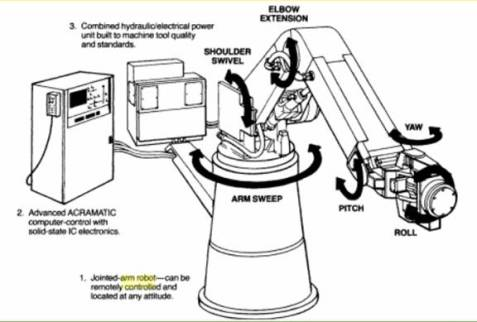
\includegraphics[width=4.3cm,height=6cm]{chapters/intro/images/t3.jpg}}\quad
\end{subfigure}
\begin{subfigure}
[Shakey]{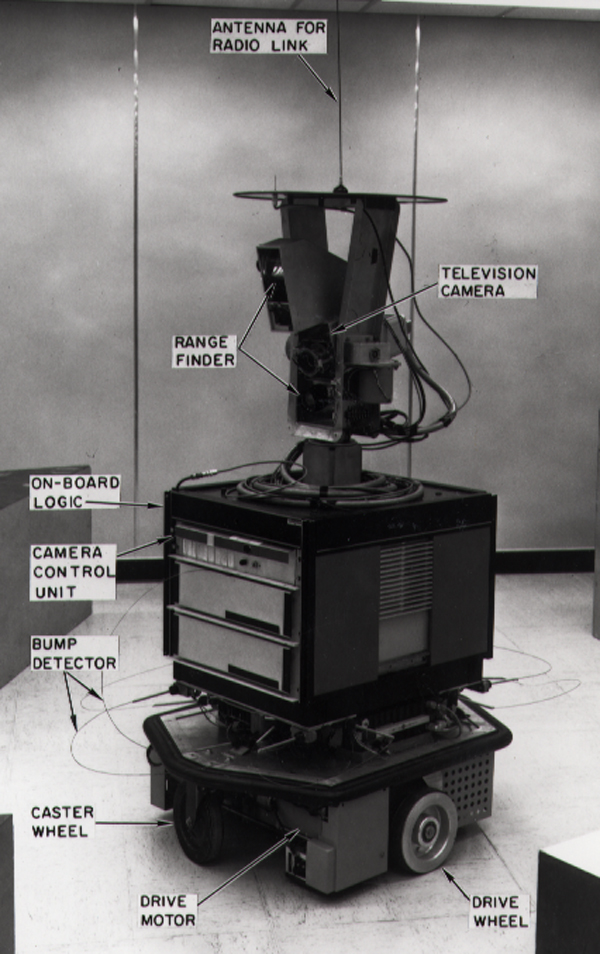
\includegraphics[width=4.1cm,height=6cm]{chapters/intro/images/Shakey.jpg}}\quad
\end{subfigure}
\begin{subfigure}
[Stanford Arm]{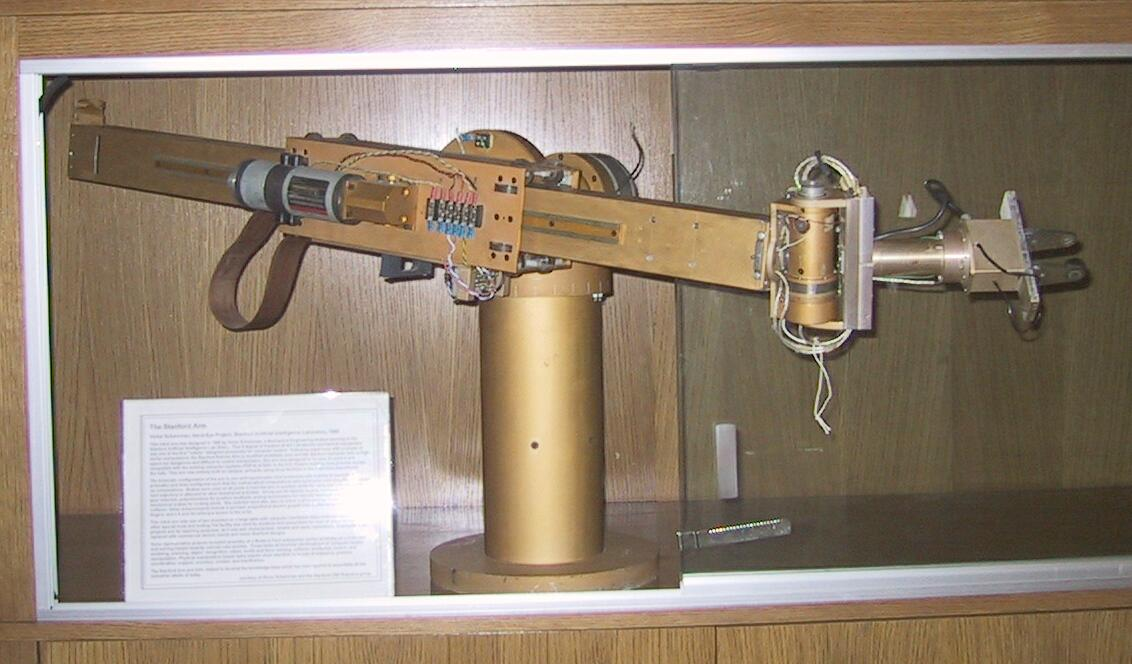
\includegraphics[width=4.1cm,height=6cm]{chapters/intro/images/stanfordarm.JPG}}\quad
\end{subfigure}
\caption{Automatons in the ancient world}
\label{fig:robots}
\end{figure}

Robotics was unanimously accepted as a key focus area to increase industrial development and achieve competitive edge. Advanced sensors such as force sensors, vision cameras and laser scanners were introduced in the late 1980s
to make physical interactions with the environment to improve the intelligence. It is necessary to make deeper connections with the control system to make intelligent decisions in the working environment. Though the vision of robotics in the 1980s was very ambitious to automise factories completely with robots and less human labour, it was very soon realized that robotics being a multi-disciplinary technology is not so easy and certain human work mechanisms are difficult to be replicated. Heterogenous integration of complex systems involves a lot of problems and developing a robotic workcells are more expensive than the workers themselves though they are economically feasible for simpler tasks.

Productivity is a complex concept and the idea of robots solely responsible for improving productivity changed in the beginning of 1990s. The dependence on robotics for more ambitious tasks started to decrease though it was and still an inevitable part of the mechatronic technology to automize and improve productivity. Now robotics are used for medical applications, service, entertainment and disaster handling applications. Though the industrial robots have been in use for quite a long time, there are many challenges not addressed until now. This is where the 'Factory in a Day' project comes into picture.

\subsection{'Factory in a Day' project}
We are aware that robot automation has been into existence since the 1960s and has seen a lot of technological advancements but they are still challenged by installation time and cost involved in setting up robots specific to the functional needs in factories. There is a lot of risk involved in such investment making it economically less attractive to smaller companies. Moreover, the factory setups are fixed environments with hard coded settings of millimeter precision so that they are perfectly under control at all times. Floating robot bases introduces errors and uncertainties which requires more robust components to handle factory scenarios. There is also a big concern in safety of human beings working in robot environments. Though recent technologies are focused towards collaborative robot control where human beings and robots can work together, these algorithms are either completely not matured to be used in factories or not yet known in the industrial community. This thesis is funded by Factory-in-a-Day project which focuses on these issues mentioned above.

Factory-in-a-Day project puts forward the idea of minimizing the installation time and the cost involved from several months to just a single day. The project focuses on the following aspects of robotics which is synonymous to the steps taken in a day to install a robotic setup. 

\begin{itemize}
\item Standardized procedures to design 3D printed custom parts which are usually attached with an existing robot arm and grippers using novel templates to minimize the time taken.
\item The flexibility to be placed in factories without any alteration where intelligent self-calibration and an adaptive framework that helps to connect with the existing machineries in ease.
\item Use rapid teaching to program production tasks in the setup from a rich set of learnable skills
for applications like mould finishing, welding and assembly.
\item Visually intuitive tools for the workers in the factory to assess robot's behavior motion behaviors. Augmented reality can be used to visualize the robot's intended path by wearing a glass to be aware of its activity to be collaborative in nature.
\item A mature human-robot interaction framework to allow the humans collaborate with robots in an unfenced workspace using a dynamic obstacle avoidance framework with proximity skin sensors and 
reactive path planning and control algorithms.
\end{itemize}
The above aspects along with proposed certification procedures and a complete focus on manufacturing industry can radically change the automation sector. The work done in this thesis orients in the direction of the last aspect which is human-robot collaboration. The Fig.~\ref{fig:doa_motivation} (a) shows the reality of many robotics based manufacturing units with fences avoiding dangerous accidents with human beings. There are strict protocols followed to get inside the fence incase of repairs needed. It is definitely not productive, and the new age robot manufacturers such as \textit{Universal Robots} focus on manufacturing robots with safe touch control which allows the robot to stop when the human is in contact. In case the robots are moving fast, they can be programmed to adapt/reduce the speed by monitoring the presence of human beings using laser scanners. Though there are systematic hacks available, the thesis supports the idea of human-robot collaboration in the real sense where they share the workspace with more awareness about the environment and task scenarios. 
\begin{figure}[!tbph]
\begin{subfigure}
[Fenced Robot for Safety]{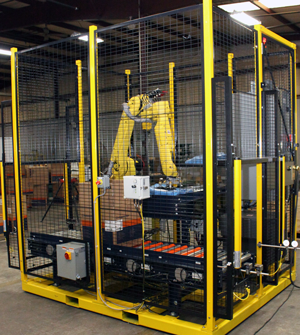
\includegraphics[width=6.6cm,height=6cm]{chapters/intro/images/fencedrobot.png}}\quad
\end{subfigure}
\begin{subfigure}
[New Gen Universal Robot]{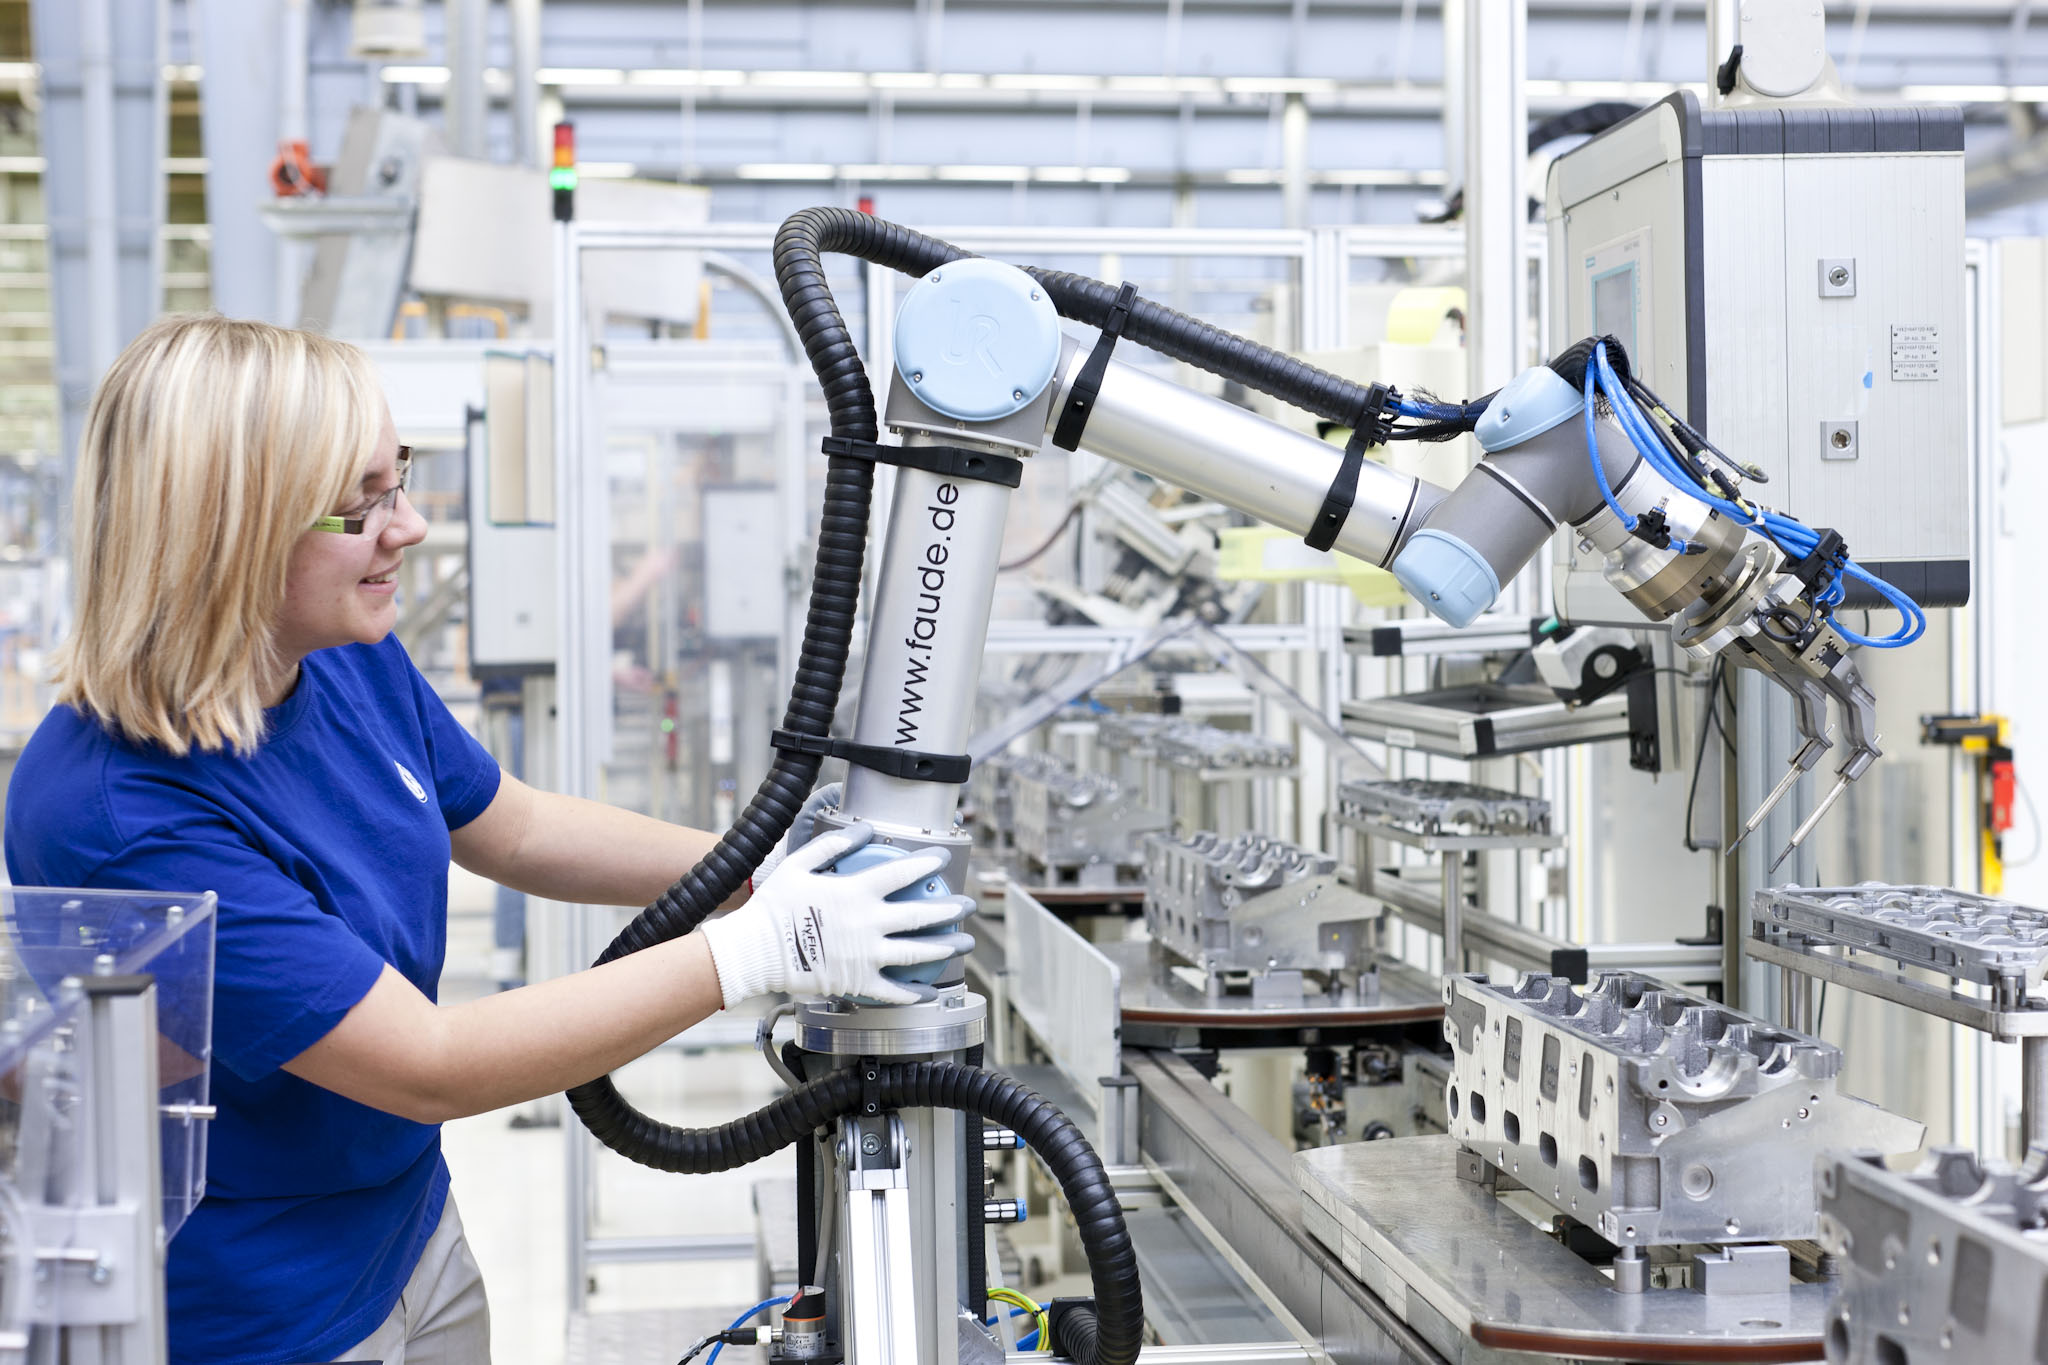
\includegraphics[width=6.5cm,height=6cm]{chapters/intro/images/urcorobot.jpg}}\quad
\end{subfigure}
\caption{Motivation towards Collaborative Robots}
\label{fig:doa_motivation}
\end{figure}
